\documentclass[1p]{elsarticle_modified}
%\bibliographystyle{elsarticle-num}

%\usepackage[colorlinks]{hyperref}
%\usepackage{abbrmath_seonhwa} %\Abb, \Ascr, \Acal ,\Abf, \Afrak
\usepackage{amsfonts}
\usepackage{amssymb}
\usepackage{amsmath}
\usepackage{amsthm}
\usepackage{scalefnt}
\usepackage{amsbsy}
\usepackage{kotex}
\usepackage{caption}
\usepackage{subfig}
\usepackage{color}
\usepackage{graphicx}
\usepackage{xcolor} %% white, black, red, green, blue, cyan, magenta, yellow
\usepackage{float}
\usepackage{setspace}
\usepackage{hyperref}

\usepackage{tikz}
\usetikzlibrary{arrows}

\usepackage{multirow}
\usepackage{array} % fixed length table
\usepackage{hhline}

%%%%%%%%%%%%%%%%%%%%%
\makeatletter
\renewcommand*\env@matrix[1][\arraystretch]{%
	\edef\arraystretch{#1}%
	\hskip -\arraycolsep
	\let\@ifnextchar\new@ifnextchar
	\array{*\c@MaxMatrixCols c}}
\makeatother %https://tex.stackexchange.com/questions/14071/how-can-i-increase-the-line-spacing-in-a-matrix
%%%%%%%%%%%%%%%

\usepackage[normalem]{ulem}

\newcommand{\msout}[1]{\ifmmode\text{\sout{\ensuremath{#1}}}\else\sout{#1}\fi}
%SOURCE: \msout is \stkout macro in https://tex.stackexchange.com/questions/20609/strikeout-in-math-mode

\newcommand{\cancel}[1]{
	\ifmmode
	{\color{red}\msout{#1}}
	\else
	{\color{red}\sout{#1}}
	\fi
}

\newcommand{\add}[1]{
	{\color{blue}\uwave{#1}}
}

\newcommand{\replace}[2]{
	\ifmmode
	{\color{red}\msout{#1}}{\color{blue}\uwave{#2}}
	\else
	{\color{red}\sout{#1}}{\color{blue}\uwave{#2}}
	\fi
}

\newcommand{\Sol}{\mathcal{S}} %segment
\newcommand{\D}{D} %diagram
\newcommand{\A}{\mathcal{A}} %arc


%%%%%%%%%%%%%%%%%%%%%%%%%%%%%5 test

\def\sl{\operatorname{\textup{SL}}(2,\Cbb)}
\def\psl{\operatorname{\textup{PSL}}(2,\Cbb)}
\def\quan{\mkern 1mu \triangleright \mkern 1mu}

\theoremstyle{definition}
\newtheorem{thm}{Theorem}[section]
\newtheorem{prop}[thm]{Proposition}
\newtheorem{lem}[thm]{Lemma}
\newtheorem{ques}[thm]{Question}
\newtheorem{cor}[thm]{Corollary}
\newtheorem{defn}[thm]{Definition}
\newtheorem{exam}[thm]{Example}
\newtheorem{rmk}[thm]{Remark}
\newtheorem{alg}[thm]{Algorithm}

\newcommand{\I}{\sqrt{-1}}
\begin{document}

%\begin{frontmatter}
%
%\title{Boundary parabolic representations of knots up to 8 crossings}
%
%%% Group authors per affiliation:
%\author{Yunhi Cho} 
%\address{Department of Mathematics, University of Seoul, Seoul, Korea}
%\ead{yhcho@uos.ac.kr}
%
%
%\author{Seonhwa Kim} %\fnref{s_kim}}
%\address{Center for Geometry and Physics, Institute for Basic Science, Pohang, 37673, Korea}
%\ead{ryeona17@ibs.re.kr}
%
%\author{Hyuk Kim}
%\address{Department of Mathematical Sciences, Seoul National University, Seoul 08826, Korea}
%\ead{hyukkim@snu.ac.kr}
%
%\author{Seokbeom Yoon}
%\address{Department of Mathematical Sciences, Seoul National University, Seoul, 08826,  Korea}
%\ead{sbyoon15@snu.ac.kr}
%
%\begin{abstract}
%We find all boundary parabolic representation of knots up to 8 crossings.
%
%\end{abstract}
%\begin{keyword}
%    \MSC[2010] 57M25 
%\end{keyword}
%
%\end{frontmatter}

%\linenumbers
%\tableofcontents
%
\newcommand\colored[1]{\textcolor{white}{\rule[-0.35ex]{0.8em}{1.4ex}}\kern-0.8em\color{red} #1}%
%\newcommand\colored[1]{\textcolor{white}{ #1}\kern-2.17ex	\textcolor{white}{ #1}\kern-1.81ex	\textcolor{white}{ #1}\kern-2.15ex\color{red}#1	}

{\Large $\underline{12n_{0641}~(K12n_{0641})}$}

\setlength{\tabcolsep}{10pt}
\renewcommand{\arraystretch}{1.6}
\vspace{1cm}\begin{tabular}{m{100pt}>{\centering\arraybackslash}m{274pt}}
\multirow{5}{120pt}{
	\centering
	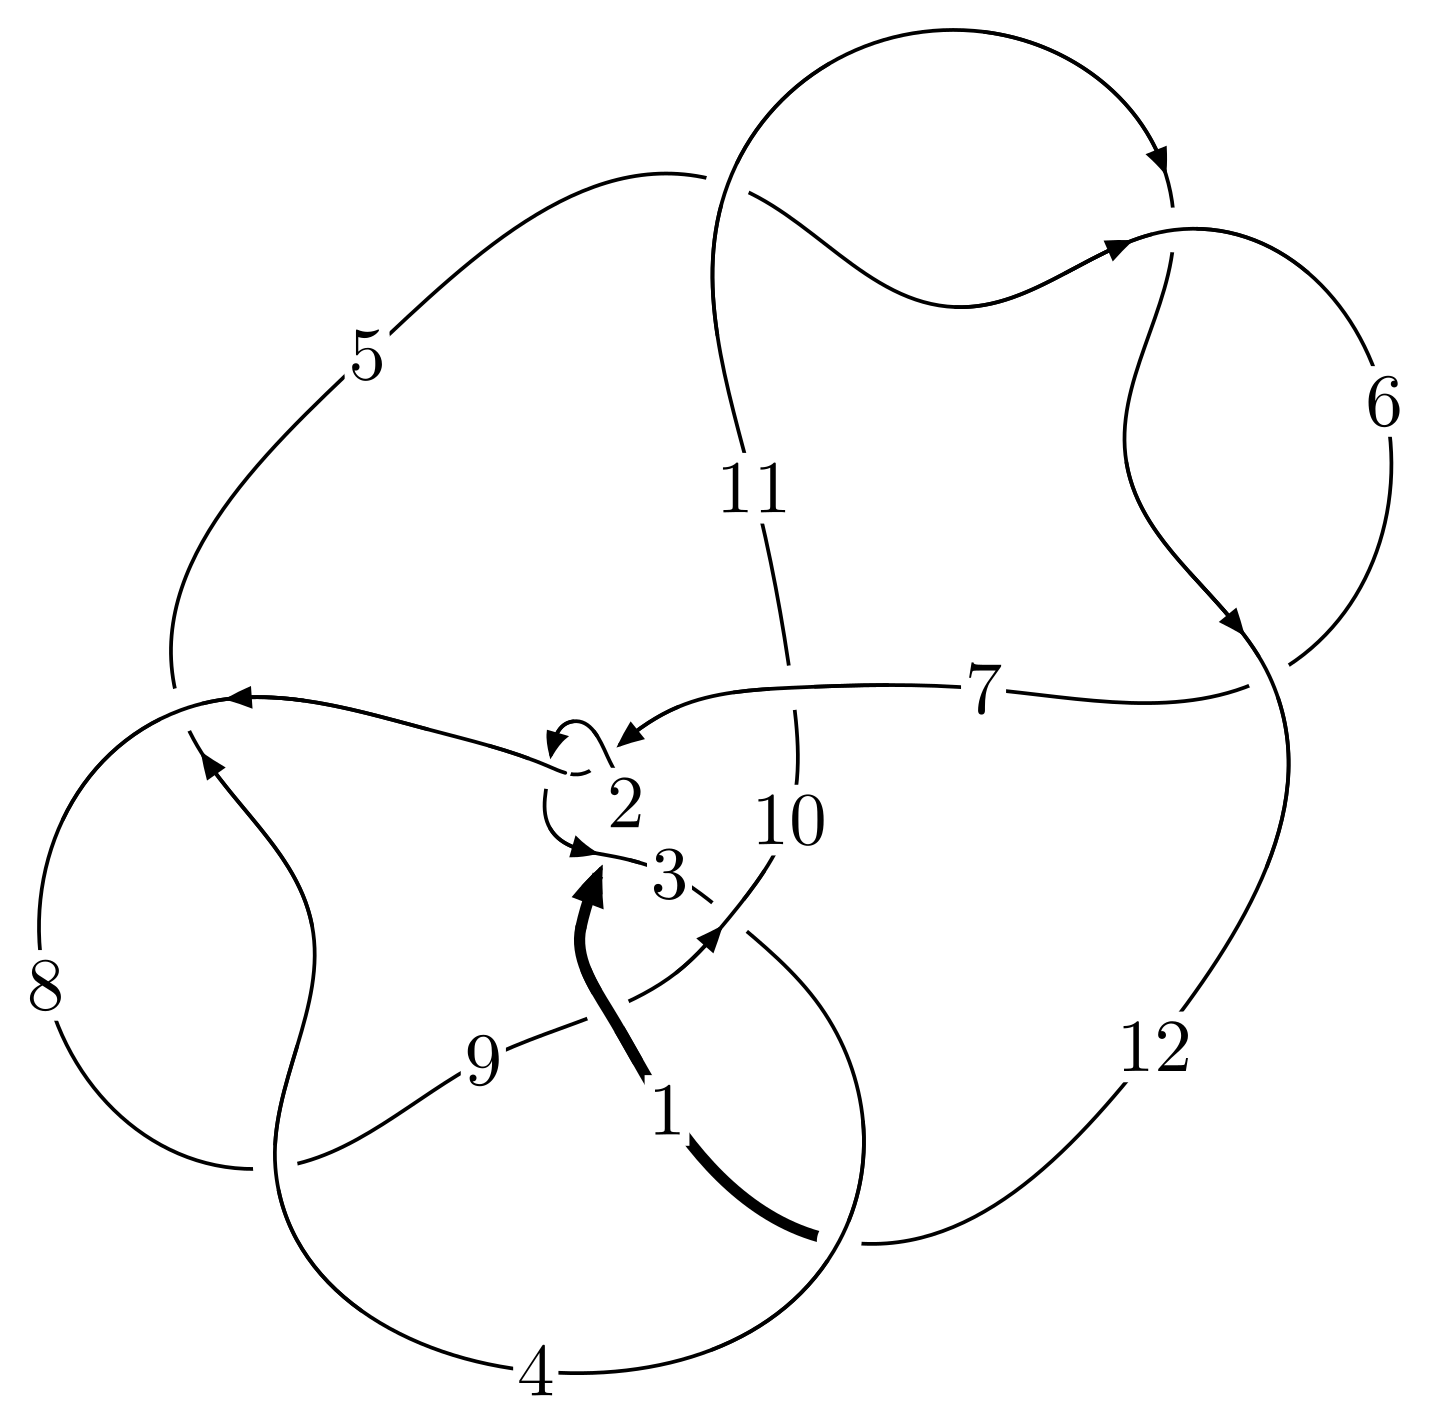
\includegraphics[width=112pt]{../../../GIT/diagram.site/Diagrams/png/2730_12n_0641.png}\\
\ \ \ A knot diagram\footnotemark}&
\allowdisplaybreaks
\textbf{Linearized knot diagam} \\
\cline{2-2}
 &
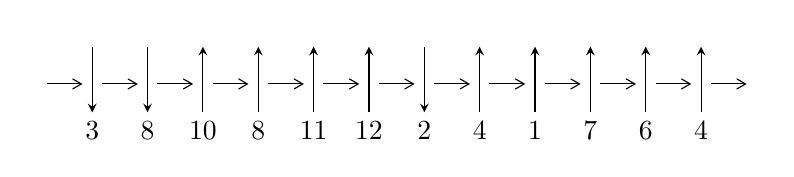
\begin{tikzpicture}[x=20pt, y=17pt]
	% nodes
	\node (C0) at (0, 0) {};
	\node (C1) at (1, 0) {};
	\node (C1U) at (1, +1) {};
	\node (C1D) at (1, -1) {3};

	\node (C2) at (2, 0) {};
	\node (C2U) at (2, +1) {};
	\node (C2D) at (2, -1) {8};

	\node (C3) at (3, 0) {};
	\node (C3U) at (3, +1) {};
	\node (C3D) at (3, -1) {10};

	\node (C4) at (4, 0) {};
	\node (C4U) at (4, +1) {};
	\node (C4D) at (4, -1) {8};

	\node (C5) at (5, 0) {};
	\node (C5U) at (5, +1) {};
	\node (C5D) at (5, -1) {11};

	\node (C6) at (6, 0) {};
	\node (C6U) at (6, +1) {};
	\node (C6D) at (6, -1) {12};

	\node (C7) at (7, 0) {};
	\node (C7U) at (7, +1) {};
	\node (C7D) at (7, -1) {2};

	\node (C8) at (8, 0) {};
	\node (C8U) at (8, +1) {};
	\node (C8D) at (8, -1) {4};

	\node (C9) at (9, 0) {};
	\node (C9U) at (9, +1) {};
	\node (C9D) at (9, -1) {1};

	\node (C10) at (10, 0) {};
	\node (C10U) at (10, +1) {};
	\node (C10D) at (10, -1) {7};

	\node (C11) at (11, 0) {};
	\node (C11U) at (11, +1) {};
	\node (C11D) at (11, -1) {6};

	\node (C12) at (12, 0) {};
	\node (C12U) at (12, +1) {};
	\node (C12D) at (12, -1) {4};
	\node (C13) at (13, 0) {};

	% arrows
	\draw[->,>={angle 60}]
	(C0) edge (C1) (C1) edge (C2) (C2) edge (C3) (C3) edge (C4) (C4) edge (C5) (C5) edge (C6) (C6) edge (C7) (C7) edge (C8) (C8) edge (C9) (C9) edge (C10) (C10) edge (C11) (C11) edge (C12) (C12) edge (C13) ;	\draw[->,>=stealth]
	(C1U) edge (C1D) (C2U) edge (C2D) (C3D) edge (C3U) (C4D) edge (C4U) (C5D) edge (C5U) (C6D) edge (C6U) (C7U) edge (C7D) (C8D) edge (C8U) (C9D) edge (C9U) (C10D) edge (C10U) (C11D) edge (C11U) (C12D) edge (C12U) ;
	\end{tikzpicture} \\
\hhline{~~} \\& 
\textbf{Solving Sequence} \\ \cline{2-2} 
 &
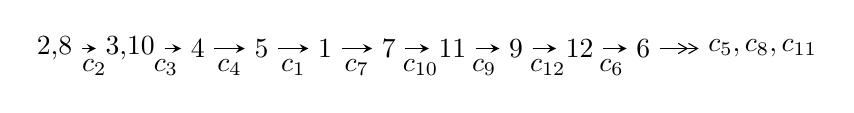
\begin{tikzpicture}[x=23pt, y=7pt]
	% node
	\node (A0) at (-1/8, 0) {2,8};
	\node (A1) at (17/16, 0) {3,10};
	\node (A2) at (17/8, 0) {4};
	\node (A3) at (25/8, 0) {5};
	\node (A4) at (33/8, 0) {1};
	\node (A5) at (41/8, 0) {7};
	\node (A6) at (49/8, 0) {11};
	\node (A7) at (57/8, 0) {9};
	\node (A8) at (65/8, 0) {12};
	\node (A9) at (73/8, 0) {6};
	\node (C1) at (1/2, -1) {$c_{2}$};
	\node (C2) at (13/8, -1) {$c_{3}$};
	\node (C3) at (21/8, -1) {$c_{4}$};
	\node (C4) at (29/8, -1) {$c_{1}$};
	\node (C5) at (37/8, -1) {$c_{7}$};
	\node (C6) at (45/8, -1) {$c_{10}$};
	\node (C7) at (53/8, -1) {$c_{9}$};
	\node (C8) at (61/8, -1) {$c_{12}$};
	\node (C9) at (69/8, -1) {$c_{6}$};
	\node (A10) at (11, 0) {$c_{5},c_{8},c_{11}$};

	% edge
	\draw[->,>=stealth]	
	(A0) edge (A1) (A1) edge (A2) (A2) edge (A3) (A3) edge (A4) (A4) edge (A5) (A5) edge (A6) (A6) edge (A7) (A7) edge (A8) (A8) edge (A9) ;
	\draw[->>,>={angle 60}]	
	(A9) edge (A10);
\end{tikzpicture} \\ 

\end{tabular} \\

\footnotetext{
The image of knot diagram is generated by the software ``\textbf{Draw programme}" developed by Andrew Bartholomew(\url{http://www.layer8.co.uk/maths/draw/index.htm\#Running-draw}), where we modified some parts for our purpose(\url{https://github.com/CATsTAILs/LinksPainter}).
}\phantom \\ \newline 
\centering \textbf{Ideals for irreducible components\footnotemark of $X_{\text{par}}$} 
 
\begin{align*}
I^u_{1}&=\langle 
8.49827\times10^{54} u^{47}+2.37919\times10^{54} u^{46}+\cdots+1.70744\times10^{55} b+8.16269\times10^{54},\\
\phantom{I^u_{1}}&\phantom{= \langle  }2.71230\times10^{55} u^{47}+6.45531\times10^{54} u^{46}+\cdots+1.70744\times10^{55} a-5.14701\times10^{56},\;u^{48}- u^{47}+\cdots+55 u-1\rangle \\
I^u_{2}&=\langle 
- u^{14}-2 u^{13}+3 u^{12}+8 u^{11}-6 u^{10}-21 u^9+5 u^8+33 u^7- u^6-36 u^5-2 u^4+22 u^3+u^2+b-8 u,\\
\phantom{I^u_{2}}&\phantom{= \langle  }-7 u^{14}-6 u^{13}+\cdots+a+9,\\
\phantom{I^u_{2}}&\phantom{= \langle  }u^{15}+u^{14}-4 u^{13}-5 u^{12}+10 u^{11}+14 u^{10}-15 u^9-25 u^8+16 u^7+28 u^6-11 u^5-19 u^4+5 u^3+7 u^2- u-1\rangle \\
I^u_{3}&=\langle 
b+1,\;a+1,\;u+1\rangle \\
\\
\end{align*}
\raggedright * 3 irreducible components of $\dim_{\mathbb{C}}=0$, with total 64 representations.\\
\footnotetext{All coefficients of polynomials are rational numbers. But the coefficients are sometimes approximated in decimal forms when there is not enough margin.}
\newpage
\renewcommand{\arraystretch}{1}
\centering \section*{I. $I^u_{1}= \langle 8.50\times10^{54} u^{47}+2.38\times10^{54} u^{46}+\cdots+1.71\times10^{55} b+8.16\times10^{54},\;2.71\times10^{55} u^{47}+6.46\times10^{54} u^{46}+\cdots+1.71\times10^{55} a-5.15\times10^{56},\;u^{48}- u^{47}+\cdots+55 u-1 \rangle$}
\flushleft \textbf{(i) Arc colorings}\\
\begin{tabular}{m{7pt} m{180pt} m{7pt} m{180pt} }
\flushright $a_{2}=$&$\begin{pmatrix}1\\0\end{pmatrix}$ \\
\flushright $a_{8}=$&$\begin{pmatrix}0\\u\end{pmatrix}$ \\
\flushright $a_{3}=$&$\begin{pmatrix}1\\u^2\end{pmatrix}$ \\
\flushright $a_{10}=$&$\begin{pmatrix}-1.58851 u^{47}-0.378069 u^{46}+\cdots+195.933 u+30.1446\\-0.497719 u^{47}-0.139342 u^{46}+\cdots+94.5690 u-0.478065\end{pmatrix}$ \\
\flushright $a_{4}=$&$\begin{pmatrix}-2.00213 u^{47}+1.12164 u^{46}+\cdots+231.824 u-45.9301\\0.532079 u^{47}-0.731391 u^{46}+\cdots+30.3920 u-2.14822\end{pmatrix}$ \\
\flushright $a_{5}=$&$\begin{pmatrix}-2.00213 u^{47}+1.12164 u^{46}+\cdots+231.824 u-45.9301\\0.836676 u^{47}-0.793694 u^{46}+\cdots-16.0332 u-1.26772\end{pmatrix}$ \\
\flushright $a_{1}=$&$\begin{pmatrix}- u^2+1\\- u^4\end{pmatrix}$ \\
\flushright $a_{7}=$&$\begin{pmatrix}u\\u\end{pmatrix}$ \\
\flushright $a_{11}=$&$\begin{pmatrix}-0.852685 u^{47}-0.569587 u^{46}+\cdots+123.900 u+31.4741\\0.238109 u^{47}-0.330861 u^{46}+\cdots+22.5362 u+0.851455\end{pmatrix}$ \\
\flushright $a_{9}=$&$\begin{pmatrix}-1.07589 u^{47}-0.438793 u^{46}+\cdots+131.390 u+30.0699\\-0.529673 u^{47}-0.199681 u^{46}+\cdots+108.525 u-0.735248\end{pmatrix}$ \\
\flushright $a_{12}=$&$\begin{pmatrix}-0.634463 u^{47}-0.0674825 u^{46}+\cdots-11.2930 u+67.9453\\-0.184246 u^{47}+0.409138 u^{46}+\cdots-14.0906 u+2.82587\end{pmatrix}$ \\
\flushright $a_{6}=$&$\begin{pmatrix}-0.0720669 u^{47}+0.836777 u^{46}+\cdots+39.2316 u-83.6537\\0.845245 u^{47}-0.416255 u^{46}+\cdots-32.8739 u-2.52326\end{pmatrix}$\\&\end{tabular}
\flushleft \textbf{(ii) Obstruction class $= -1$}\\~\\
\flushleft \textbf{(iii) Cusp Shapes $= 5.23094 u^{47}-3.23434 u^{46}+\cdots-404.902 u+24.1944$}\\~\\
\newpage\renewcommand{\arraystretch}{1}
\flushleft \textbf{(iv) u-Polynomials at the component}\newline \\
\begin{tabular}{m{50pt}|m{274pt}}
Crossings & \hspace{64pt}u-Polynomials at each crossing \\
\hline $$\begin{aligned}c_{1}\end{aligned}$$&$\begin{aligned}
&u^{48}+15 u^{47}+\cdots+2837 u+1
\end{aligned}$\\
\hline $$\begin{aligned}c_{2},c_{7}\end{aligned}$$&$\begin{aligned}
&u^{48}+u^{47}+\cdots-55 u-1
\end{aligned}$\\
\hline $$\begin{aligned}c_{3}\end{aligned}$$&$\begin{aligned}
&u^{48}+u^{47}+\cdots-14 u+1
\end{aligned}$\\
\hline $$\begin{aligned}c_{4},c_{8}\end{aligned}$$&$\begin{aligned}
&u^{48}-2 u^{47}+\cdots+14560 u+15853
\end{aligned}$\\
\hline $$\begin{aligned}c_{5},c_{6},c_{11}\end{aligned}$$&$\begin{aligned}
&u^{48}+2 u^{47}+\cdots-12 u-1
\end{aligned}$\\
\hline $$\begin{aligned}c_{9}\end{aligned}$$&$\begin{aligned}
&u^{48}+u^{47}+\cdots+719 u-293
\end{aligned}$\\
\hline $$\begin{aligned}c_{10}\end{aligned}$$&$\begin{aligned}
&u^{48}-3 u^{47}+\cdots+10344 u+649
\end{aligned}$\\
\hline $$\begin{aligned}c_{12}\end{aligned}$$&$\begin{aligned}
&u^{48}+4 u^{47}+\cdots-10508 u-1369
\end{aligned}$\\
\hline
\end{tabular}\\~\\
\newpage\renewcommand{\arraystretch}{1}
\flushleft \textbf{(v) Riley Polynomials at the component}\newline \\
\begin{tabular}{m{50pt}|m{274pt}}
Crossings & \hspace{64pt}Riley Polynomials at each crossing \\
\hline $$\begin{aligned}c_{1}\end{aligned}$$&$\begin{aligned}
&y^{48}+53 y^{47}+\cdots-7937733 y+1
\end{aligned}$\\
\hline $$\begin{aligned}c_{2},c_{7}\end{aligned}$$&$\begin{aligned}
&y^{48}-15 y^{47}+\cdots-2837 y+1
\end{aligned}$\\
\hline $$\begin{aligned}c_{3}\end{aligned}$$&$\begin{aligned}
&y^{48}+5 y^{47}+\cdots-56 y+1
\end{aligned}$\\
\hline $$\begin{aligned}c_{4},c_{8}\end{aligned}$$&$\begin{aligned}
&y^{48}-64 y^{47}+\cdots-8556537210 y+251317609
\end{aligned}$\\
\hline $$\begin{aligned}c_{5},c_{6},c_{11}\end{aligned}$$&$\begin{aligned}
&y^{48}-50 y^{47}+\cdots-66 y+1
\end{aligned}$\\
\hline $$\begin{aligned}c_{9}\end{aligned}$$&$\begin{aligned}
&y^{48}-61 y^{47}+\cdots-3226039 y+85849
\end{aligned}$\\
\hline $$\begin{aligned}c_{10}\end{aligned}$$&$\begin{aligned}
&y^{48}-39 y^{47}+\cdots-45579572 y+421201
\end{aligned}$\\
\hline $$\begin{aligned}c_{12}\end{aligned}$$&$\begin{aligned}
&y^{48}-60 y^{47}+\cdots-53809914 y+1874161
\end{aligned}$\\
\hline
\end{tabular}\\~\\
\newpage\flushleft \textbf{(vi) Complex Volumes and Cusp Shapes}
$$\begin{array}{c|c|c}  
\text{Solutions to }I^u_{1}& \I (\text{vol} + \sqrt{-1}CS) & \text{Cusp shape}\\
 \hline 
\begin{aligned}
u &= \phantom{-}0.780489 + 0.693178 I \\
a &= \phantom{-}0.705695 - 0.209382 I \\
b &= \phantom{-}0.862042 + 0.604842 I\end{aligned}
 & -0.43674 - 2.43309 I & \phantom{-}6.83450 + 4.39555 I \\ \hline\begin{aligned}
u &= \phantom{-}0.780489 - 0.693178 I \\
a &= \phantom{-}0.705695 + 0.209382 I \\
b &= \phantom{-}0.862042 - 0.604842 I\end{aligned}
 & -0.43674 + 2.43309 I & \phantom{-}6.83450 - 4.39555 I \\ \hline\begin{aligned}
u &= \phantom{-}0.529535 + 0.795568 I \\
a &= \phantom{-}1.41726 + 0.21633 I \\
b &= \phantom{-}0.20894 + 1.50824 I\end{aligned}
 & \phantom{-}7.15738 + 1.35453 I & \phantom{-}12.13081 - 1.57989 I \\ \hline\begin{aligned}
u &= \phantom{-}0.529535 - 0.795568 I \\
a &= \phantom{-}1.41726 - 0.21633 I \\
b &= \phantom{-}0.20894 - 1.50824 I\end{aligned}
 & \phantom{-}7.15738 - 1.35453 I & \phantom{-}12.13081 + 1.57989 I \\ \hline\begin{aligned}
u &= -1.052950 + 0.007832 I \\
a &= -0.707699 + 0.058294 I \\
b &= -0.965617 + 0.004183 I\end{aligned}
 & \phantom{-}1.65094 + 0.00093 I & \phantom{-}6.00000 + 0.11555 I \\ \hline\begin{aligned}
u &= -1.052950 - 0.007832 I \\
a &= -0.707699 - 0.058294 I \\
b &= -0.965617 - 0.004183 I\end{aligned}
 & \phantom{-}1.65094 - 0.00093 I & \phantom{-}6.00000 - 0.11555 I \\ \hline\begin{aligned}
u &= \phantom{-}1.05847\phantom{ +0.000000I} \\
a &= \phantom{-}1.90687\phantom{ +0.000000I} \\
b &= \phantom{-}3.40742\phantom{ +0.000000I}\end{aligned}
 & \phantom{-}8.27045\phantom{ +0.000000I} & \phantom{-}10.2350\phantom{ +0.000000I} \\ \hline\begin{aligned}
u &= \phantom{-}0.912791 + 0.183084 I \\
a &= -1.080850 - 0.514657 I \\
b &= -1.221840 + 0.446864 I\end{aligned}
 & -0.81244 - 3.97179 I & \phantom{-}3.30801 + 3.48283 I \\ \hline\begin{aligned}
u &= \phantom{-}0.912791 - 0.183084 I \\
a &= -1.080850 + 0.514657 I \\
b &= -1.221840 - 0.446864 I\end{aligned}
 & -0.81244 + 3.97179 I & \phantom{-}3.30801 - 3.48283 I \\ \hline\begin{aligned}
u &= \phantom{-}0.918294 + 0.651222 I \\
a &= -0.957067 - 0.032883 I \\
b &= -0.745662 - 0.216607 I\end{aligned}
 & -1.09728 - 2.73985 I & \phantom{-}8.74885 + 1.99555 I\\
 \hline 
 \end{array}$$\newpage$$\begin{array}{c|c|c}  
\text{Solutions to }I^u_{1}& \I (\text{vol} + \sqrt{-1}CS) & \text{Cusp shape}\\
 \hline 
\begin{aligned}
u &= \phantom{-}0.918294 - 0.651222 I \\
a &= -0.957067 + 0.032883 I \\
b &= -0.745662 + 0.216607 I\end{aligned}
 & -1.09728 + 2.73985 I & \phantom{-}8.74885 - 1.99555 I \\ \hline\begin{aligned}
u &= -1.064190 + 0.512825 I \\
a &= \phantom{-}1.060480 - 0.792956 I \\
b &= \phantom{-}0.694905 - 1.218350 I\end{aligned}
 & -0.91409 + 4.62733 I & \phantom{-}6.00000 - 9.84335 I \\ \hline\begin{aligned}
u &= -1.064190 - 0.512825 I \\
a &= \phantom{-}1.060480 + 0.792956 I \\
b &= \phantom{-}0.694905 + 1.218350 I\end{aligned}
 & -0.91409 - 4.62733 I & \phantom{-}6.00000 + 9.84335 I \\ \hline\begin{aligned}
u &= -0.798516 + 0.871376 I \\
a &= -1.77948 + 0.85153 I \\
b &= \phantom{-}0.462172 + 1.321260 I\end{aligned}
 & \phantom{-}14.6213 + 0.5837 I & \phantom{-}11.01767 + 0. I\phantom{ +0.000000I} \\ \hline\begin{aligned}
u &= -0.798516 - 0.871376 I \\
a &= -1.77948 - 0.85153 I \\
b &= \phantom{-}0.462172 - 1.321260 I\end{aligned}
 & \phantom{-}14.6213 - 0.5837 I & \phantom{-}11.01767 + 0. I\phantom{ +0.000000I} \\ \hline\begin{aligned}
u &= \phantom{-}0.846297 + 0.834975 I \\
a &= -0.598082 - 0.641634 I \\
b &= -0.31678 - 1.81032 I\end{aligned}
 & \phantom{-}7.53406 - 1.71339 I & \phantom{-}6.00000 + 0. I\phantom{ +0.000000I} \\ \hline\begin{aligned}
u &= \phantom{-}0.846297 - 0.834975 I \\
a &= -0.598082 + 0.641634 I \\
b &= -0.31678 + 1.81032 I\end{aligned}
 & \phantom{-}7.53406 + 1.71339 I & \phantom{-}6.00000 + 0. I\phantom{ +0.000000I} \\ \hline\begin{aligned}
u &= -0.717176 + 0.997613 I \\
a &= \phantom{-}0.584667 - 0.723750 I \\
b &= -0.218697 - 1.389430 I\end{aligned}
 & \phantom{-}7.96025 - 3.20779 I & \phantom{-0.000000 } 0 \\ \hline\begin{aligned}
u &= -0.717176 - 0.997613 I \\
a &= \phantom{-}0.584667 + 0.723750 I \\
b &= -0.218697 + 1.389430 I\end{aligned}
 & \phantom{-}7.96025 + 3.20779 I & \phantom{-0.000000 } 0 \\ \hline\begin{aligned}
u &= -0.734348 + 0.989945 I \\
a &= -0.626011 - 0.351788 I \\
b &= -0.795948 + 0.818156 I\end{aligned}
 & \phantom{-}4.61963 + 5.43773 I & \phantom{-0.000000 } 0\\
 \hline 
 \end{array}$$\newpage$$\begin{array}{c|c|c}  
\text{Solutions to }I^u_{1}& \I (\text{vol} + \sqrt{-1}CS) & \text{Cusp shape}\\
 \hline 
\begin{aligned}
u &= -0.734348 - 0.989945 I \\
a &= -0.626011 + 0.351788 I \\
b &= -0.795948 - 0.818156 I\end{aligned}
 & \phantom{-}4.61963 - 5.43773 I & \phantom{-0.000000 } 0 \\ \hline\begin{aligned}
u &= \phantom{-}0.958511 + 0.797758 I \\
a &= \phantom{-}1.47360 + 0.69247 I \\
b &= \phantom{-}0.338863 + 1.303150 I\end{aligned}
 & \phantom{-}7.17999 - 4.40128 I & \phantom{-0.000000 } 0 \\ \hline\begin{aligned}
u &= \phantom{-}0.958511 - 0.797758 I \\
a &= \phantom{-}1.47360 - 0.69247 I \\
b &= \phantom{-}0.338863 - 1.303150 I\end{aligned}
 & \phantom{-}7.17999 + 4.40128 I & \phantom{-0.000000 } 0 \\ \hline\begin{aligned}
u &= \phantom{-}1.177050 + 0.420372 I \\
a &= -0.180221 - 0.366873 I \\
b &= -0.0135532 + 0.0338086 I\end{aligned}
 & -1.66489 - 2.36125 I & \phantom{-0.000000 } 0 \\ \hline\begin{aligned}
u &= \phantom{-}1.177050 - 0.420372 I \\
a &= -0.180221 + 0.366873 I \\
b &= -0.0135532 - 0.0338086 I\end{aligned}
 & -1.66489 + 2.36125 I & \phantom{-0.000000 } 0 \\ \hline\begin{aligned}
u &= \phantom{-}1.076140 + 0.640039 I \\
a &= -1.46685 - 0.95325 I \\
b &= -0.59898 - 2.24608 I\end{aligned}
 & \phantom{-}5.49499 - 6.77666 I & \phantom{-0.000000 } 0 \\ \hline\begin{aligned}
u &= \phantom{-}1.076140 - 0.640039 I \\
a &= -1.46685 + 0.95325 I \\
b &= -0.59898 + 2.24608 I\end{aligned}
 & \phantom{-}5.49499 + 6.77666 I & \phantom{-0.000000 } 0 \\ \hline\begin{aligned}
u &= -0.724809 + 1.033950 I \\
a &= \phantom{-}1.064180 + 0.400574 I \\
b &= \phantom{-}0.486196 - 0.793628 I\end{aligned}
 & \phantom{-}4.91559 + 3.36660 I & \phantom{-0.000000 } 0 \\ \hline\begin{aligned}
u &= -0.724809 - 1.033950 I \\
a &= \phantom{-}1.064180 - 0.400574 I \\
b &= \phantom{-}0.486196 + 0.793628 I\end{aligned}
 & \phantom{-}4.91559 - 3.36660 I & \phantom{-0.000000 } 0 \\ \hline\begin{aligned}
u &= -0.712486\phantom{ +0.000000I} \\
a &= -1.97788\phantom{ +0.000000I} \\
b &= -2.16627\phantom{ +0.000000I}\end{aligned}
 & \phantom{-}2.80010\phantom{ +0.000000I} & -4.83520\phantom{ +0.000000I}\\
 \hline 
 \end{array}$$\newpage$$\begin{array}{c|c|c}  
\text{Solutions to }I^u_{1}& \I (\text{vol} + \sqrt{-1}CS) & \text{Cusp shape}\\
 \hline 
\begin{aligned}
u &= -1.014230 + 0.800845 I \\
a &= \phantom{-}0.675996 - 0.593941 I \\
b &= \phantom{-}0.53182 - 2.37364 I\end{aligned}
 & \phantom{-}13.9471 + 5.6591 I & \phantom{-0.000000 } 0 \\ \hline\begin{aligned}
u &= -1.014230 - 0.800845 I \\
a &= \phantom{-}0.675996 + 0.593941 I \\
b &= \phantom{-}0.53182 + 2.37364 I\end{aligned}
 & \phantom{-}13.9471 - 5.6591 I & \phantom{-0.000000 } 0 \\ \hline\begin{aligned}
u &= -0.694037 + 0.060458 I \\
a &= \phantom{-}1.24961 - 1.05080 I \\
b &= \phantom{-}0.696219 + 0.640293 I\end{aligned}
 & -4.12135 + 0.22643 I & \phantom{-}0.431456 + 0.910944 I \\ \hline\begin{aligned}
u &= -0.694037 - 0.060458 I \\
a &= \phantom{-}1.24961 + 1.05080 I \\
b &= \phantom{-}0.696219 - 0.640293 I\end{aligned}
 & -4.12135 - 0.22643 I & \phantom{-}0.431456 - 0.910944 I \\ \hline\begin{aligned}
u &= -0.414437 + 0.505333 I \\
a &= -0.950768 + 0.151291 I \\
b &= -0.409586 + 0.582781 I\end{aligned}
 & \phantom{-}0.970583 - 0.357083 I & \phantom{-}10.29975 + 3.20108 I \\ \hline\begin{aligned}
u &= -0.414437 - 0.505333 I \\
a &= -0.950768 - 0.151291 I \\
b &= -0.409586 - 0.582781 I\end{aligned}
 & \phantom{-}0.970583 + 0.357083 I & \phantom{-}10.29975 - 3.20108 I \\ \hline\begin{aligned}
u &= -1.086260 + 0.818808 I \\
a &= -1.40570 + 0.48518 I \\
b &= -0.89489 + 1.58340 I\end{aligned}
 & \phantom{-}6.79477 + 9.83464 I & \phantom{-0.000000 } 0 \\ \hline\begin{aligned}
u &= -1.086260 - 0.818808 I \\
a &= -1.40570 - 0.48518 I \\
b &= -0.89489 - 1.58340 I\end{aligned}
 & \phantom{-}6.79477 - 9.83464 I & \phantom{-0.000000 } 0 \\ \hline\begin{aligned}
u &= \phantom{-}0.602545 + 0.150612 I \\
a &= -0.74027 + 2.02291 I \\
b &= -0.480320 - 0.677791 I\end{aligned}
 & \phantom{-}0.44759 - 3.90440 I & \phantom{-}6.22150 + 4.06117 I \\ \hline\begin{aligned}
u &= \phantom{-}0.602545 - 0.150612 I \\
a &= -0.74027 - 2.02291 I \\
b &= -0.480320 + 0.677791 I\end{aligned}
 & \phantom{-}0.44759 + 3.90440 I & \phantom{-}6.22150 - 4.06117 I\\
 \hline 
 \end{array}$$\newpage$$\begin{array}{c|c|c}  
\text{Solutions to }I^u_{1}& \I (\text{vol} + \sqrt{-1}CS) & \text{Cusp shape}\\
 \hline 
\begin{aligned}
u &= \phantom{-}0.587564\phantom{ +0.000000I} \\
a &= \phantom{-}6.68300\phantom{ +0.000000I} \\
b &= \phantom{-}2.00737\phantom{ +0.000000I}\end{aligned}
 & \phantom{-}10.3493\phantom{ +0.000000I} & -7.38360\phantom{ +0.000000I} \\ \hline\begin{aligned}
u &= \phantom{-}0.748414 + 1.199110 I \\
a &= -0.608875 - 0.775844 I \\
b &= \phantom{-}0.92843 - 1.37321 I\end{aligned}
 & \phantom{-}14.9212 + 6.6040 I & \phantom{-0.000000 } 0 \\ \hline\begin{aligned}
u &= \phantom{-}0.748414 - 1.199110 I \\
a &= -0.608875 + 0.775844 I \\
b &= \phantom{-}0.92843 + 1.37321 I\end{aligned}
 & \phantom{-}14.9212 - 6.6040 I & \phantom{-0.000000 } 0 \\ \hline\begin{aligned}
u &= \phantom{-}1.17568 + 0.88106 I \\
a &= \phantom{-}1.43185 + 0.33117 I \\
b &= \phantom{-}1.26045 + 2.00959 I\end{aligned}
 & \phantom{-}13.4534 - 14.0241 I & \phantom{-0.000000 } 0 \\ \hline\begin{aligned}
u &= \phantom{-}1.17568 - 0.88106 I \\
a &= \phantom{-}1.43185 - 0.33117 I \\
b &= \phantom{-}1.26045 - 2.00959 I\end{aligned}
 & \phantom{-}13.4534 + 14.0241 I & \phantom{-0.000000 } 0 \\ \hline\begin{aligned}
u &= -1.40098 + 0.67383 I \\
a &= \phantom{-}0.295089 + 0.214824 I \\
b &= \phantom{-}0.930979 + 0.758020 I\end{aligned}
 & \phantom{-}2.75175 + 3.73669 I & \phantom{-0.000000 } 0 \\ \hline\begin{aligned}
u &= -1.40098 - 0.67383 I \\
a &= \phantom{-}0.295089 - 0.214824 I \\
b &= \phantom{-}0.930979 - 0.758020 I\end{aligned}
 & \phantom{-}2.75175 - 3.73669 I & \phantom{-0.000000 } 0 \\ \hline\begin{aligned}
u &= \phantom{-}0.0188398\phantom{ +0.000000I} \\
a &= \phantom{-}33.6749\phantom{ +0.000000I} \\
b &= \phantom{-}1.27318\phantom{ +0.000000I}\end{aligned}
 & \phantom{-}6.34803\phantom{ +0.000000I} & \phantom{-}16.5030\phantom{ +0.000000I}\\
 \hline 
 \end{array}$$\newpage\newpage\renewcommand{\arraystretch}{1}
\centering \section*{II. $I^u_{2}= \langle - u^{14}-2 u^{13}+\cdots+b-8 u,\;-7 u^{14}-6 u^{13}+\cdots+a+9,\;u^{15}+u^{14}+\cdots- u-1 \rangle$}
\flushleft \textbf{(i) Arc colorings}\\
\begin{tabular}{m{7pt} m{180pt} m{7pt} m{180pt} }
\flushright $a_{2}=$&$\begin{pmatrix}1\\0\end{pmatrix}$ \\
\flushright $a_{8}=$&$\begin{pmatrix}0\\u\end{pmatrix}$ \\
\flushright $a_{3}=$&$\begin{pmatrix}1\\u^2\end{pmatrix}$ \\
\flushright $a_{10}=$&$\begin{pmatrix}7 u^{14}+6 u^{13}+\cdots+25 u-9\\u^{14}+2 u^{13}+\cdots- u^2+8 u\end{pmatrix}$ \\
\flushright $a_{4}=$&$\begin{pmatrix}u^{14}-5 u^{12}+\cdots+2 u-7\\-4 u^{14}-4 u^{13}+\cdots-5 u-1\end{pmatrix}$ \\
\flushright $a_{5}=$&$\begin{pmatrix}u^{14}-5 u^{12}+\cdots+2 u-7\\-4 u^{14}-4 u^{13}+\cdots-6 u^2-5 u\end{pmatrix}$ \\
\flushright $a_{1}=$&$\begin{pmatrix}- u^2+1\\- u^4\end{pmatrix}$ \\
\flushright $a_{7}=$&$\begin{pmatrix}u\\u\end{pmatrix}$ \\
\flushright $a_{11}=$&$\begin{pmatrix}6 u^{14}+6 u^{13}+\cdots+21 u-7\\2 u^{13}+2 u^{12}+\cdots+4 u+2\end{pmatrix}$ \\
\flushright $a_{9}=$&$\begin{pmatrix}6 u^{14}+5 u^{13}+\cdots+19 u-8\\u^{14}+2 u^{13}+\cdots- u^2+8 u\end{pmatrix}$ \\
\flushright $a_{12}=$&$\begin{pmatrix}- u^{14}+5 u^{12}+\cdots-2 u+8\\5 u^{14}+4 u^{13}+\cdots+15 u^2+8 u\end{pmatrix}$ \\
\flushright $a_{6}=$&$\begin{pmatrix}-8 u^{14}-2 u^{13}+\cdots-16 u+18\\-6 u^{14}- u^{13}+\cdots-8 u+9\end{pmatrix}$\\&\end{tabular}
\flushleft \textbf{(ii) Obstruction class $= 1$}\\~\\
\flushleft \textbf{(iii) Cusp Shapes $= -12 u^{14}+58 u^{12}+12 u^{11}-169 u^{10}-44 u^9+317 u^8+107 u^7-433 u^6-113 u^5+392 u^4+65 u^3-214 u^2-6 u+58$}\\~\\
\newpage\renewcommand{\arraystretch}{1}
\flushleft \textbf{(iv) u-Polynomials at the component}\newline \\
\begin{tabular}{m{50pt}|m{274pt}}
Crossings & \hspace{64pt}u-Polynomials at each crossing \\
\hline $$\begin{aligned}c_{1}\end{aligned}$$&$\begin{aligned}
&u^{15}-9 u^{14}+\cdots+15 u-1
\end{aligned}$\\
\hline $$\begin{aligned}c_{2}\end{aligned}$$&$\begin{aligned}
&u^{15}+u^{14}+\cdots- u-1
\end{aligned}$\\
\hline $$\begin{aligned}c_{3}\end{aligned}$$&$\begin{aligned}
&u^{15}+4 u^{13}+\cdots-3 u^2-1
\end{aligned}$\\
\hline $$\begin{aligned}c_{4}\end{aligned}$$&$\begin{aligned}
&u^{15}+3 u^{13}+\cdots+4 u^2+1
\end{aligned}$\\
\hline $$\begin{aligned}c_{5},c_{6}\end{aligned}$$&$\begin{aligned}
&u^{15}-8 u^{13}+\cdots-12 u^3-1
\end{aligned}$\\
\hline $$\begin{aligned}c_{7}\end{aligned}$$&$\begin{aligned}
&u^{15}- u^{14}+\cdots- u+1
\end{aligned}$\\
\hline $$\begin{aligned}c_{8}\end{aligned}$$&$\begin{aligned}
&u^{15}+3 u^{13}+\cdots-4 u^2-1
\end{aligned}$\\
\hline $$\begin{aligned}c_{9}\end{aligned}$$&$\begin{aligned}
&u^{15}- u^{14}+\cdots- u+1
\end{aligned}$\\
\hline $$\begin{aligned}c_{10}\end{aligned}$$&$\begin{aligned}
&u^{15}-8 u^{12}+\cdots-3 u^2+1
\end{aligned}$\\
\hline $$\begin{aligned}c_{11}\end{aligned}$$&$\begin{aligned}
&u^{15}-8 u^{13}+\cdots-12 u^3+1
\end{aligned}$\\
\hline $$\begin{aligned}c_{12}\end{aligned}$$&$\begin{aligned}
&u^{15}- u^{13}+\cdots+4 u^2+1
\end{aligned}$\\
\hline
\end{tabular}\\~\\
\newpage\renewcommand{\arraystretch}{1}
\flushleft \textbf{(v) Riley Polynomials at the component}\newline \\
\begin{tabular}{m{50pt}|m{274pt}}
Crossings & \hspace{64pt}Riley Polynomials at each crossing \\
\hline $$\begin{aligned}c_{1}\end{aligned}$$&$\begin{aligned}
&y^{15}+11 y^{14}+\cdots+31 y-1
\end{aligned}$\\
\hline $$\begin{aligned}c_{2},c_{7}\end{aligned}$$&$\begin{aligned}
&y^{15}-9 y^{14}+\cdots+15 y-1
\end{aligned}$\\
\hline $$\begin{aligned}c_{3}\end{aligned}$$&$\begin{aligned}
&y^{15}+8 y^{14}+\cdots-6 y-1
\end{aligned}$\\
\hline $$\begin{aligned}c_{4},c_{8}\end{aligned}$$&$\begin{aligned}
&y^{15}+6 y^{14}+\cdots-8 y-1
\end{aligned}$\\
\hline $$\begin{aligned}c_{5},c_{6},c_{11}\end{aligned}$$&$\begin{aligned}
&y^{15}-16 y^{14}+\cdots+12 y^2-1
\end{aligned}$\\
\hline $$\begin{aligned}c_{9}\end{aligned}$$&$\begin{aligned}
&y^{15}-15 y^{14}+\cdots+9 y-1
\end{aligned}$\\
\hline $$\begin{aligned}c_{10}\end{aligned}$$&$\begin{aligned}
&y^{15}-22 y^{13}+\cdots+6 y-1
\end{aligned}$\\
\hline $$\begin{aligned}c_{12}\end{aligned}$$&$\begin{aligned}
&y^{15}-2 y^{14}+\cdots-8 y-1
\end{aligned}$\\
\hline
\end{tabular}\\~\\
\newpage\flushleft \textbf{(vi) Complex Volumes and Cusp Shapes}
$$\begin{array}{c|c|c}  
\text{Solutions to }I^u_{2}& \I (\text{vol} + \sqrt{-1}CS) & \text{Cusp shape}\\
 \hline 
\begin{aligned}
u &= -0.894768 + 0.381504 I \\
a &= \phantom{-}0.561192 - 0.613047 I \\
b &= -0.133265 + 0.484278 I\end{aligned}
 & -3.89584 + 1.58539 I & \phantom{-}2.11826 - 3.74447 I \\ \hline\begin{aligned}
u &= -0.894768 - 0.381504 I \\
a &= \phantom{-}0.561192 + 0.613047 I \\
b &= -0.133265 - 0.484278 I\end{aligned}
 & -3.89584 - 1.58539 I & \phantom{-}2.11826 + 3.74447 I \\ \hline\begin{aligned}
u &= \phantom{-}1.002760 + 0.378711 I \\
a &= -0.492433 - 0.387786 I \\
b &= -0.380671 + 0.657450 I\end{aligned}
 & -0.33265 - 5.51163 I & \phantom{-}4.94815 + 7.40556 I \\ \hline\begin{aligned}
u &= \phantom{-}1.002760 - 0.378711 I \\
a &= -0.492433 + 0.387786 I \\
b &= -0.380671 - 0.657450 I\end{aligned}
 & -0.33265 + 5.51163 I & \phantom{-}4.94815 - 7.40556 I \\ \hline\begin{aligned}
u &= \phantom{-}0.800420 + 0.321515 I \\
a &= -0.433427 - 0.987439 I \\
b &= \phantom{-}0.703055 + 0.417003 I\end{aligned}
 & \phantom{-}0.48032 + 2.56256 I & \phantom{-}7.50726 + 0.32927 I \\ \hline\begin{aligned}
u &= \phantom{-}0.800420 - 0.321515 I \\
a &= -0.433427 + 0.987439 I \\
b &= \phantom{-}0.703055 - 0.417003 I\end{aligned}
 & \phantom{-}0.48032 - 2.56256 I & \phantom{-}7.50726 - 0.32927 I \\ \hline\begin{aligned}
u &= -0.712036\phantom{ +0.000000I} \\
a &= -1.36567\phantom{ +0.000000I} \\
b &= -2.13667\phantom{ +0.000000I}\end{aligned}
 & \phantom{-}5.68620\phantom{ +0.000000I} & \phantom{-}3.34500\phantom{ +0.000000I} \\ \hline\begin{aligned}
u &= \phantom{-}1.083910 + 0.722936 I \\
a &= -0.725633 - 0.017802 I \\
b &= -0.738745 - 0.392095 I\end{aligned}
 & -1.62262 - 3.23030 I & -0.70757 + 9.71898 I \\ \hline\begin{aligned}
u &= \phantom{-}1.083910 - 0.722936 I \\
a &= -0.725633 + 0.017802 I \\
b &= -0.738745 + 0.392095 I\end{aligned}
 & -1.62262 + 3.23030 I & -0.70757 - 9.71898 I \\ \hline\begin{aligned}
u &= -0.945359 + 0.963665 I \\
a &= \phantom{-}0.814338 + 0.249756 I \\
b &= \phantom{-}0.603655 - 0.873044 I\end{aligned}
 & \phantom{-}3.65766 + 5.39923 I & \phantom{-}5.36277 - 6.12141 I\\
 \hline 
 \end{array}$$\newpage$$\begin{array}{c|c|c}  
\text{Solutions to }I^u_{2}& \I (\text{vol} + \sqrt{-1}CS) & \text{Cusp shape}\\
 \hline 
\begin{aligned}
u &= -0.945359 - 0.963665 I \\
a &= \phantom{-}0.814338 - 0.249756 I \\
b &= \phantom{-}0.603655 + 0.873044 I\end{aligned}
 & \phantom{-}3.65766 - 5.39923 I & \phantom{-}5.36277 + 6.12141 I \\ \hline\begin{aligned}
u &= \phantom{-}0.620323\phantom{ +0.000000I} \\
a &= \phantom{-}2.57729\phantom{ +0.000000I} \\
b &= \phantom{-}2.00007\phantom{ +0.000000I}\end{aligned}
 & \phantom{-}3.14873\phantom{ +0.000000I} & \phantom{-}19.3840\phantom{ +0.000000I} \\ \hline\begin{aligned}
u &= -1.268280 + 0.578450 I \\
a &= \phantom{-}0.548163 - 0.056389 I \\
b &= \phantom{-}1.152480 - 0.111993 I\end{aligned}
 & \phantom{-}1.86244 + 1.54512 I & \phantom{-}7.16780 - 3.17961 I \\ \hline\begin{aligned}
u &= -1.268280 - 0.578450 I \\
a &= \phantom{-}0.548163 + 0.056389 I \\
b &= \phantom{-}1.152480 + 0.111993 I\end{aligned}
 & \phantom{-}1.86244 - 1.54512 I & \phantom{-}7.16780 + 3.17961 I \\ \hline\begin{aligned}
u &= -0.465662\phantom{ +0.000000I} \\
a &= -7.75602\phantom{ +0.000000I} \\
b &= -2.27641\phantom{ +0.000000I}\end{aligned}
 & \phantom{-}10.6056\phantom{ +0.000000I} & \phantom{-}24.4780\phantom{ +0.000000I}\\
 \hline 
 \end{array}$$\newpage\newpage\renewcommand{\arraystretch}{1}
\centering \section*{III. $I^u_{3}= \langle b+1,\;a+1,\;u+1 \rangle$}
\flushleft \textbf{(i) Arc colorings}\\
\begin{tabular}{m{7pt} m{180pt} m{7pt} m{180pt} }
\flushright $a_{2}=$&$\begin{pmatrix}1\\0\end{pmatrix}$ \\
\flushright $a_{8}=$&$\begin{pmatrix}0\\-1\end{pmatrix}$ \\
\flushright $a_{3}=$&$\begin{pmatrix}1\\1\end{pmatrix}$ \\
\flushright $a_{10}=$&$\begin{pmatrix}-1\\-1\end{pmatrix}$ \\
\flushright $a_{4}=$&$\begin{pmatrix}1\\1\end{pmatrix}$ \\
\flushright $a_{5}=$&$\begin{pmatrix}1\\0\end{pmatrix}$ \\
\flushright $a_{1}=$&$\begin{pmatrix}0\\-1\end{pmatrix}$ \\
\flushright $a_{7}=$&$\begin{pmatrix}-1\\-1\end{pmatrix}$ \\
\flushright $a_{11}=$&$\begin{pmatrix}-1\\-1\end{pmatrix}$ \\
\flushright $a_{9}=$&$\begin{pmatrix}-1\\-2\end{pmatrix}$ \\
\flushright $a_{12}=$&$\begin{pmatrix}1\\0\end{pmatrix}$ \\
\flushright $a_{6}=$&$\begin{pmatrix}0\\-1\end{pmatrix}$\\&\end{tabular}
\flushleft \textbf{(ii) Obstruction class $= -1$}\\~\\
\flushleft \textbf{(iii) Cusp Shapes $= 6$}\\~\\
\newpage\renewcommand{\arraystretch}{1}
\flushleft \textbf{(iv) u-Polynomials at the component}\newline \\
\begin{tabular}{m{50pt}|m{274pt}}
Crossings & \hspace{64pt}u-Polynomials at each crossing \\
\hline $$\begin{aligned}c_{1},c_{12}\end{aligned}$$&$\begin{aligned}
&u+1
\end{aligned}$\\
\hline $$\begin{aligned}c_{2},c_{4},c_{5}\\c_{6},c_{7},c_{8}\\c_{9},c_{11}\end{aligned}$$&$\begin{aligned}
&u-1
\end{aligned}$\\
\hline $$\begin{aligned}c_{3},c_{10}\end{aligned}$$&$\begin{aligned}
&u
\end{aligned}$\\
\hline
\end{tabular}\\~\\
\newpage\renewcommand{\arraystretch}{1}
\flushleft \textbf{(v) Riley Polynomials at the component}\newline \\
\begin{tabular}{m{50pt}|m{274pt}}
Crossings & \hspace{64pt}Riley Polynomials at each crossing \\
\hline $$\begin{aligned}c_{1},c_{2},c_{4}\\c_{5},c_{6},c_{7}\\c_{8},c_{9},c_{11}\\c_{12}\end{aligned}$$&$\begin{aligned}
&y-1
\end{aligned}$\\
\hline $$\begin{aligned}c_{3},c_{10}\end{aligned}$$&$\begin{aligned}
&y
\end{aligned}$\\
\hline
\end{tabular}\\~\\
\newpage\flushleft \textbf{(vi) Complex Volumes and Cusp Shapes}
$$\begin{array}{c|c|c}  
\text{Solutions to }I^u_{3}& \I (\text{vol} + \sqrt{-1}CS) & \text{Cusp shape}\\
 \hline 
\begin{aligned}
u &= -1.00000\phantom{ +0.000000I} \\
a &= -1.00000\phantom{ +0.000000I} \\
b &= -1.00000\phantom{ +0.000000I}\end{aligned}
 & \phantom{-}1.64493\phantom{ +0.000000I} & \phantom{-}6.00000\phantom{ +0.000000I}\\
 \hline 
 \end{array}$$\newpage
\newpage\renewcommand{\arraystretch}{1}
\centering \section*{ IV. u-Polynomials}
\begin{tabular}{m{50pt}|m{274pt}}
Crossings & \hspace{64pt}u-Polynomials at each crossing \\
\hline $$\begin{aligned}c_{1}\end{aligned}$$&$\begin{aligned}
&(u+1)(u^{15}-9 u^{14}+\cdots+15 u-1)(u^{48}+15 u^{47}+\cdots+2837 u+1)
\end{aligned}$\\
\hline $$\begin{aligned}c_{2}\end{aligned}$$&$\begin{aligned}
&(u-1)(u^{15}+u^{14}+\cdots- u-1)(u^{48}+u^{47}+\cdots-55 u-1)
\end{aligned}$\\
\hline $$\begin{aligned}c_{3}\end{aligned}$$&$\begin{aligned}
&u(u^{15}+4 u^{13}+\cdots-3 u^2-1)(u^{48}+u^{47}+\cdots-14 u+1)
\end{aligned}$\\
\hline $$\begin{aligned}c_{4}\end{aligned}$$&$\begin{aligned}
&(u-1)(u^{15}+3 u^{13}+\cdots+4 u^2+1)(u^{48}-2 u^{47}+\cdots+14560 u+15853)
\end{aligned}$\\
\hline $$\begin{aligned}c_{5},c_{6}\end{aligned}$$&$\begin{aligned}
&(u-1)(u^{15}-8 u^{13}+\cdots-12 u^3-1)(u^{48}+2 u^{47}+\cdots-12 u-1)
\end{aligned}$\\
\hline $$\begin{aligned}c_{7}\end{aligned}$$&$\begin{aligned}
&(u-1)(u^{15}- u^{14}+\cdots- u+1)(u^{48}+u^{47}+\cdots-55 u-1)
\end{aligned}$\\
\hline $$\begin{aligned}c_{8}\end{aligned}$$&$\begin{aligned}
&(u-1)(u^{15}+3 u^{13}+\cdots-4 u^2-1)(u^{48}-2 u^{47}+\cdots+14560 u+15853)
\end{aligned}$\\
\hline $$\begin{aligned}c_{9}\end{aligned}$$&$\begin{aligned}
&(u-1)(u^{15}- u^{14}+\cdots- u+1)(u^{48}+u^{47}+\cdots+719 u-293)
\end{aligned}$\\
\hline $$\begin{aligned}c_{10}\end{aligned}$$&$\begin{aligned}
&u(u^{15}-8 u^{12}+\cdots-3 u^2+1)(u^{48}-3 u^{47}+\cdots+10344 u+649)
\end{aligned}$\\
\hline $$\begin{aligned}c_{11}\end{aligned}$$&$\begin{aligned}
&(u-1)(u^{15}-8 u^{13}+\cdots-12 u^3+1)(u^{48}+2 u^{47}+\cdots-12 u-1)
\end{aligned}$\\
\hline $$\begin{aligned}c_{12}\end{aligned}$$&$\begin{aligned}
&(u+1)(u^{15}- u^{13}+\cdots+4 u^2+1)(u^{48}+4 u^{47}+\cdots-10508 u-1369)
\end{aligned}$\\
\hline
\end{tabular}\newpage\renewcommand{\arraystretch}{1}
\centering \section*{ V. Riley Polynomials}
\begin{tabular}{m{50pt}|m{274pt}}
Crossings & \hspace{64pt}Riley Polynomials at each crossing \\
\hline $$\begin{aligned}c_{1}\end{aligned}$$&$\begin{aligned}
&(y-1)(y^{15}+11 y^{14}+\cdots+31 y-1)(y^{48}+53 y^{47}+\cdots-7937733 y+1)
\end{aligned}$\\
\hline $$\begin{aligned}c_{2},c_{7}\end{aligned}$$&$\begin{aligned}
&(y-1)(y^{15}-9 y^{14}+\cdots+15 y-1)(y^{48}-15 y^{47}+\cdots-2837 y+1)
\end{aligned}$\\
\hline $$\begin{aligned}c_{3}\end{aligned}$$&$\begin{aligned}
&y(y^{15}+8 y^{14}+\cdots-6 y-1)(y^{48}+5 y^{47}+\cdots-56 y+1)
\end{aligned}$\\
\hline $$\begin{aligned}c_{4},c_{8}\end{aligned}$$&$\begin{aligned}
&(y-1)(y^{15}+6 y^{14}+\cdots-8 y-1)\\
&\cdot(y^{48}-64 y^{47}+\cdots-8556537210 y+251317609)
\end{aligned}$\\
\hline $$\begin{aligned}c_{5},c_{6},c_{11}\end{aligned}$$&$\begin{aligned}
&(y-1)(y^{15}-16 y^{14}+\cdots+12 y^2-1)(y^{48}-50 y^{47}+\cdots-66 y+1)
\end{aligned}$\\
\hline $$\begin{aligned}c_{9}\end{aligned}$$&$\begin{aligned}
&(y-1)(y^{15}-15 y^{14}+\cdots+9 y-1)\\
&\cdot(y^{48}-61 y^{47}+\cdots-3226039 y+85849)
\end{aligned}$\\
\hline $$\begin{aligned}c_{10}\end{aligned}$$&$\begin{aligned}
&y(y^{15}-22 y^{13}+\cdots+6 y-1)\\
&\cdot(y^{48}-39 y^{47}+\cdots-45579572 y+421201)
\end{aligned}$\\
\hline $$\begin{aligned}c_{12}\end{aligned}$$&$\begin{aligned}
&(y-1)(y^{15}-2 y^{14}+\cdots-8 y-1)\\
&\cdot(y^{48}-60 y^{47}+\cdots-53809914 y+1874161)
\end{aligned}$\\
\hline
\end{tabular}
\vskip 2pc
\end{document}